%----------------------------------------------------------------------------
\chapter{\docker}
%----------------------------------------------------------------------------
\section{Monolitikus alkalmazásokról a mikroszolgáltatásokra való áttérés}
A monolitikus alkalmazások olyan komponensekből állnak, amelyek mindegyike szorosan összekapcsolt és egyetlen egységként kell fejleszteni, telepíteni és kezelni, mivel mind egyetlen rendszerfolyamatként futnak.
Az alkalmazás egy részének módosítása az egész alkalmazás újratelepítését igényli, és idővel a részek közötti határok hiánya a részek közötti korlátlanul növekvő komplexitáshoz és következésképpen az egész rendszer minőségének romlásához vezet, mivel a részek közötti függőségek korlátlanul növekednek.
A rendszer növekvő terhelésének kezeléséhez vagy vertikálisan kell skálázni a szervereket több processzor, memória és egyéb szerverelem hozzáadásával, vagy horizontálisan kell skálázni az egész rendszert további szerverek felállításával és az alkalmazás több példányának futtatásával.
Bár a vertikális skálázás általában nem igényel semmilyen változtatást az alkalmazáson, viszonylag gyorsan drágul, és a gyakorlatban mindig van egy felső korlátja.
A horizontális skálázás viszont viszonylag olcsó hardveresen, de nagy változtatásokat igényelhet az alkalmazás kódjában, és nem mindig lehetséges - az alkalmazás bizonyos részei rendkívül nehezen vagy szinte lehetetlenül horizontálisan skálázni (például relációs adatbázisok).
Ha egy monolitikus alkalmazás bármely része nem skálázható, akkor az egész alkalmazás skálázhatatlan lesz, hacsak nem lehet valahogy felosztani a monolitot.

\begin{figure}[ht]
    \centering
         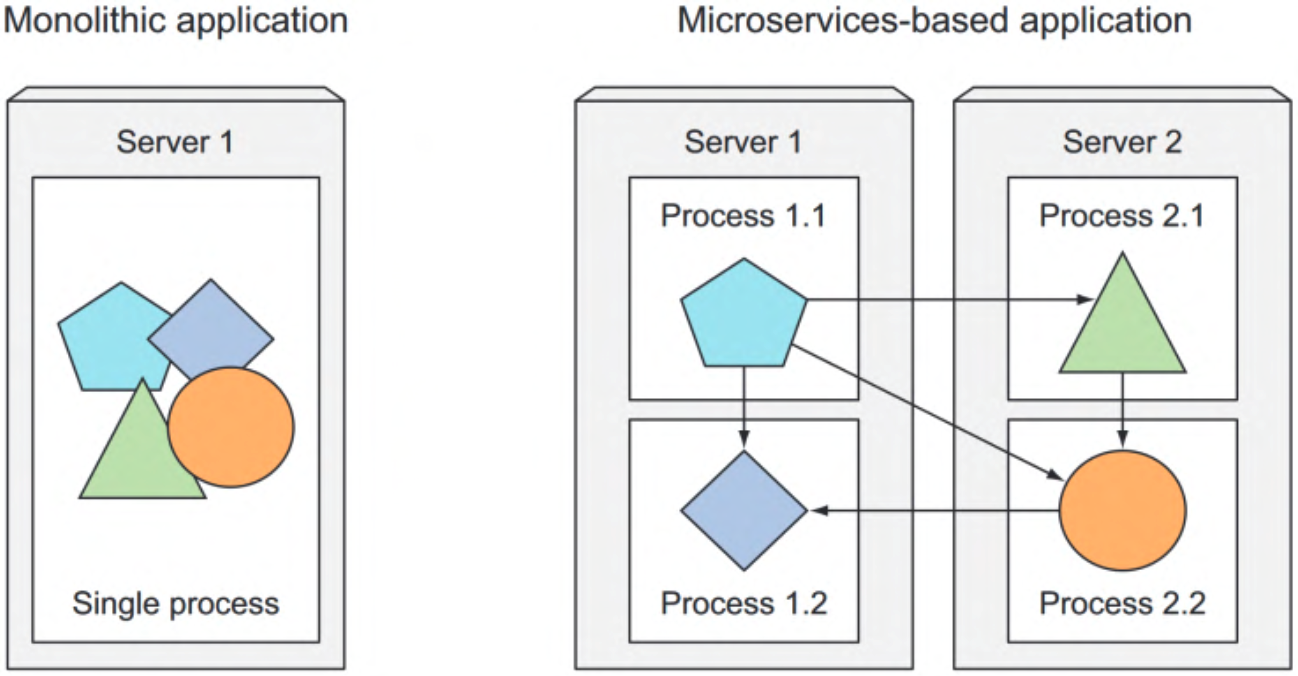
\includegraphics[width=0.85\textwidth]{figures/docker/monolithic-and-microservices.png}
          \caption{Komponensek egy monolitikus alkalmazáson belül és az önálló mikroszolgáltatások összehasonlítása \cite{Marko17}.}
           \label{monolithic-and-microservices}
\end{figure}

Ezek és más problémák arra kényszerítettek minket, hogy elkezdjük az összetett monolitikus alkalmazásokat kisebb, egymástól függetlenül telepíthető komponensekre, úgynevezett mikroszolgáltatásokra bontani.
Minden mikroszolgáltatás önálló folyamatként fut (lásd \ref{monolithic-and-microservices} ábrán), és egyszerű, jól definiált interfészeken (API-kon) keresztül kommunikál más mikroszolgáltatásokkal \cite{Marko17}.

\section{Konténerek előnyei}
Ahelyett, hogy virtuális gépeket használnának az egyes mikroszolgáltatások környezetének elkülönítésére, a fejlesztők a Linux konténertechnológiákhoz fordulnak.
Ezek lehetővé teszik, hogy több szolgáltatást futtassanak ugyanazon a számítógépen, miközben nem csak más környezetet állítanak fel mindegyiknek, hanem el is szigetelik őket egymástól, hasonlóan a virtuálisgépekhez, de sokkal kevesebb pazarlással (lásd \ref{vm-vs-containers} ábrán).
Egy konténerben futó folyamat a számítógép operációs rendszerén belül fut, mint az összes többi folyamat (ellentétben a virtuálisgépekkel, ahol a folyamatok külön operációs rendszerben futnak).
A konténerben lévő folyamat azonban továbbra is el van szigetelve a többi folyamattól.
Magának a folyamatnak úgy tűnik, mintha csak ő futna a gépen és annak operációs rendszerében \cite{Marko17}.

\begin{figure}[ht]
    \centering
         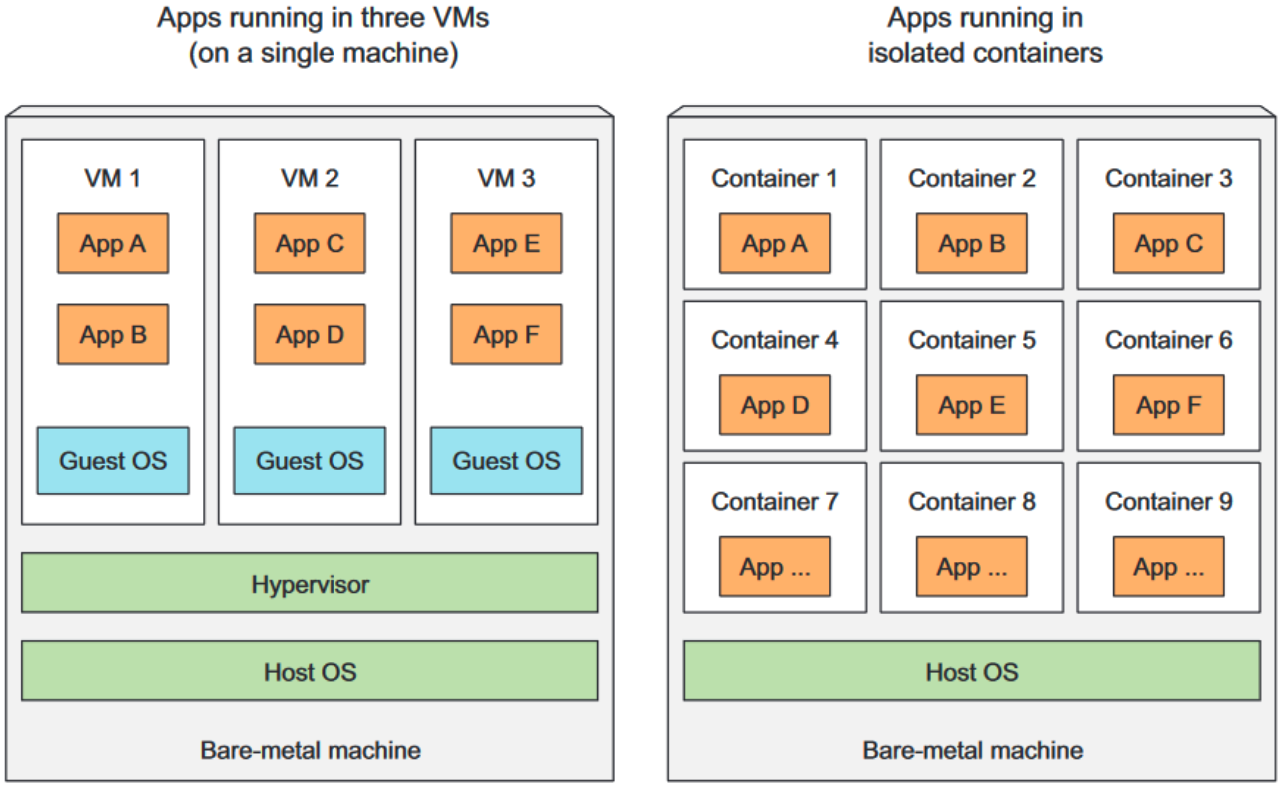
\includegraphics[width=0.9\textwidth]{figures/docker/vm-vs-containers.png}
          \caption{Virtuálisgépek használata alkalmazáscsoportok elkülönítésére és az egyes alkalmazások elkülönítése konténerekkel való illusztrálása \cite{Marko17}.}
           \label{vm-vs-containers}
\end{figure}

\section{Docker platform}
Bár a konténertechnológiák már régóta léteznek, a Docker konténerplatform elterjedésével váltak szélesebb körben ismertté.
A Docker volt az első konténerrendszer, amely a konténereket könnyen hordozhatóvá tette különböző gépek között.
Leegyszerűsítette azt a folyamatot, hogy nem csak az alkalmazást, hanem annak összes könyvtárát és egyéb függőségét, sőt a teljes operációs rendszer fájlrendszerét is egy egyszerű, hordozható csomagba csomagolja, amellyel az alkalmazás bármely más, Dockert futtató gépen elérhetővé tehető (lásd \ref{running-containers} ábrán).
A Docker-alapú konténerképek rétegekből állnak, amelyek több képen is megoszthatók és újrafelhasználhatók.
Ez azt jelenti, hogy egy képnek csak bizonyos rétegeit kell letölteni, ha a többi réteg már korábban letöltésre került egy másik konténer futtatása során, amely ugyanezeket a rétegeket tartalmazza \cite{Marko17}.

\begin{figure}[ht]
    \centering
         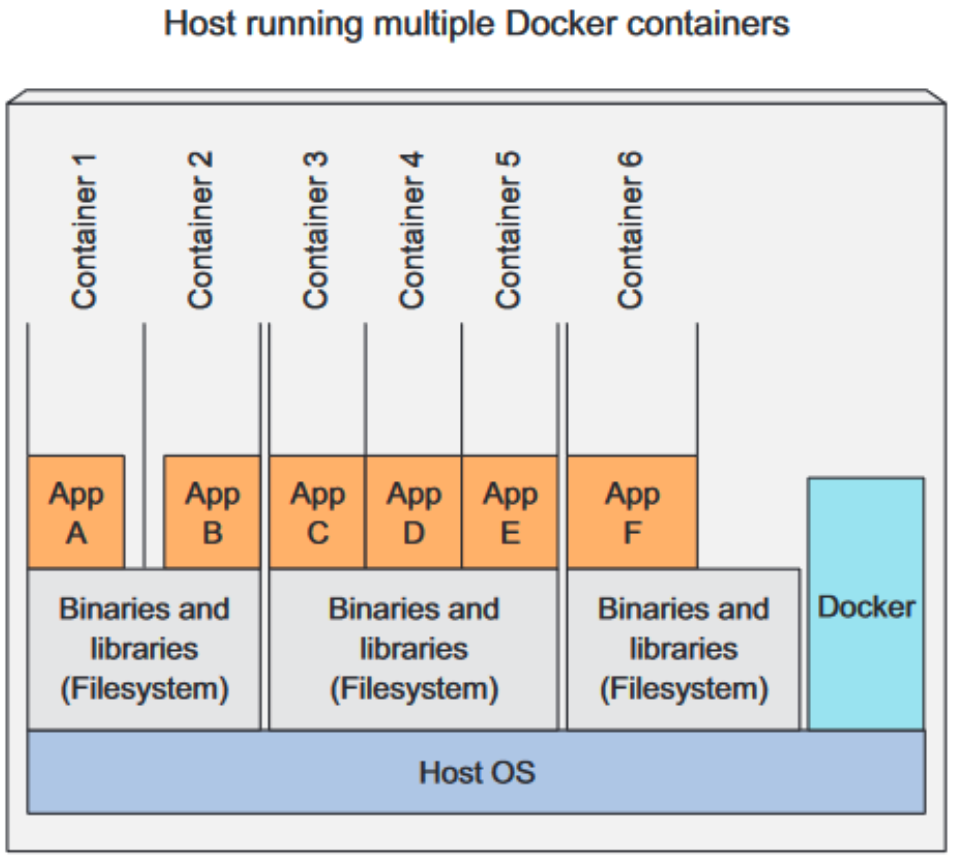
\includegraphics[width=0.65\textwidth]{figures/docker/running-contaiers.png}
          \caption{Docker konténerek használatának ábrázolása \cite{Marko17}.}
           \label{running-containers}
\end{figure}